\documentclass[german=true,thesistype=bachelor,proposal]{tubsthesis}

\usepackage{lipsum}
\usepackage{pgfgantt} % Schedule

\thesisname{Johanna Doe}
\thesismatrikel{1234567}
\thesisemail{j.doe@tu-braunschweig.de}
\thesismajor{Informatik}
\thesisduration{3}
\thesissupervisors{Super Visor, M. Sc.}{Dr. Dipper Visor}{}
\thesisprofessor[Prof.\,Dr.-Ing.\,Jane Smith]{Prof.\,Dr.-Ing.\,Lars Eisbär}
\thesistitle{Titel der Thesis}{Title of the thesis}
\thesisbegindate{2020-01-01}
%\thesisenddate{2020-01-02}
\thesispresentationpoints{5.7}

\addbibresource{bibliography.bib}

\thesisinstitute{Institut für Perfektes Schreiben in IT}

\begin{document}
\begin{thesis}

\chapter{Einleitung und Motivation} % English: Introduction and Motivation
\lipsum

\chapter{Verwandte Arbeiten} % English: Related Work
\lipsum[1-3]

\begin{figure}
\centering
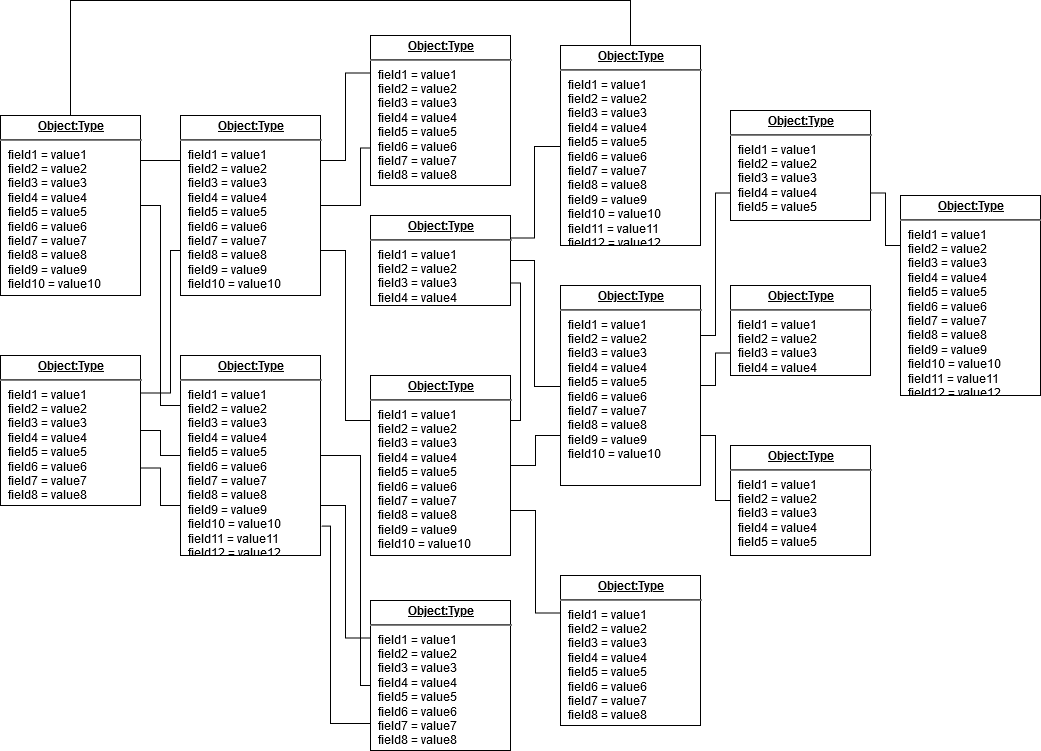
\includegraphics[width=\textwidth]{images/example_diagram.png}
\caption{Ein Diagramm, nicht relevant für irgendetwas~\cite{lisa}}
\label{fig:inga}
\end{figure}

\lipsum[4-5]

\chapter{Aufgabenstellung} % English: Task
\lipsum[1-3]

\chapter{Evaluation} % English: Evaluation
\lipsum[1-4]

\chapter{Zeitplan} % English: Schedule

% für Masterarbeiten / for Master's Theses
Für Masterarbeiten:\\
\begin{ganttchart}[hgrid, vgrid,]{1}{24}
\gantttitle{Woche}{24} \\
\gantttitlelist{1,...,24}{1} \\
\ganttbar{AP1}{1}{4} \\
\ganttbar{AP2}{5}{9} \\
\ganttmilestone{Meilenstein}{6} \\ % Meilenstein nach 6 Wochen / milestone after 6 weeks
\ganttmilestone{Zwischenvortrag}{6} \\ % Zwischenvortrag nur bei Masterarbeiten / intermediate presentation only for Master's Theses
\ganttbar{AP3}{7}{17} \\
\ganttbar{AP4}{18}{23} \\
\ganttbar{Druck und Abgabe}{24}{24} \\
\ganttmilestone{Abschlussvortrag}{24}
\end{ganttchart}

% für Bachelorarbeiten / for Bachelor's Theses
Für Bachelorarbeiten:\\
\begin{ganttchart}[hgrid, vgrid,]{1}{12}
\gantttitle{Woche}{12} \\
\gantttitlelist{1,...,12}{1} \\
\ganttbar{AP1}{1}{4} \\
\ganttbar{AP2}{5}{9} \\
\ganttbar{AP3}{7}{11} \\
\ganttbar{Druck und Abgabe}{12}{12} \\
\ganttmilestone{Abschlussvortrag}{12}
\end{ganttchart}

\section{Arbeitspakete} % English: Work Packages
Jedes Arbeitspaket wird genau beschrieben.
Jedes Arbeitspaket bekommt eine stichpunktartige Liste von Muss- und Kann-Kriterien,
deren Erfüllung später überprüfbar ist.

% Each work package is described precisely.
% Each work packages has a bullet point list of mandatory and optional criteria
% that can be verified later.
\lipsum[4]

\subsection{AP1: ...} % English: WP1: ...
\lipsum[1]

\subsection{AP2: ...} % English: WP2: ...
\lipsum[2]

\subsection{AP3: ...} % English: WP3: ...
\lipsum[3]

\section{Meilenstein} % English: Milestones
nur bei Masterarbeiten
Hier wird aufgelistet, welche Kriterien bis zum Meilenstein erfüllt sein müssen.
Für Arbeitspakete die über den Meilenstein hinaus gehen (hier etwa AP2) müssen die Kriterien
genau beschrieben sein, die am Meilenstein erfüllt sind.

% only for Master's Theses
% Please list here, which criteria have to be fulfilled until the milestone is reached.
% For work packages that outlast the milestone (here WP2) the criteria,
% that will be fulfilled at the milestone, have to be described precisely.

\lipsum[5]

\end{thesis}
\end{document}